%=========================================================
\chapter{Planeación del Tiempo}	
\label{cap:tiempo}

	Este capítulo presenta el desglose de la planeación del tiempo del proyecto, contiene la lista de actividades, entregables y esfuerzo requerido para el proyecto, así como las metodologías a utilizar.

%---------------------------------------------------------
\section{Metodología de desarrollo}

\cdtInstrucciones{
	Liste o describa las metodologías a aplicar en el proyecto y como se combinarán o de que forma se aplicarán.
}

%---------------------------------------------------------
\section{Descomposición de tareas}	

\cdtInstrucciones{
	Tabla con la lista de actividades mediante la técnica de WorkBreakDown Structure.
}

\begin{table}[hbtp!]
    \noindent\begin{tabular}{|p{.05\textwidth}|p{.65\textwidth}|p{.1\textwidth}|p{.1\textwidth}|}
    	\hline
    	{\bf Id} & {\bf Nombre} & {\bf Esfuerzo} & {\bf Dep.} \\
    	\hline
    	T1 & Entrevista con el cliente. & 4hrs. & - \\
    	\hline
    	T2 & Identificación de requerimientos. & 2 días. & T1 \\
    	\hline
    	T3 & Instalar entorno de desarrollo. & 1 día & - \\
    	\hline
    	T4 & Definir numero de Sprints y alcance. & 2 dias.. & T2 \\
    	\hline
    	T5 & Hacer el Product Backlog & 1 día. & T2, T3 \\
    	\hline
    	... & ... & ... & ... \\
    	\hline
    \end{tabular}
	\caption{Lista de estructura de trabajo.}
	\label{tbl:wbs}
\end{table}

%---------------------------------------------------------
\section{Diagrama de Gantt}

\begin{figure}[htbp!]
	\begin{center}
		\fbox{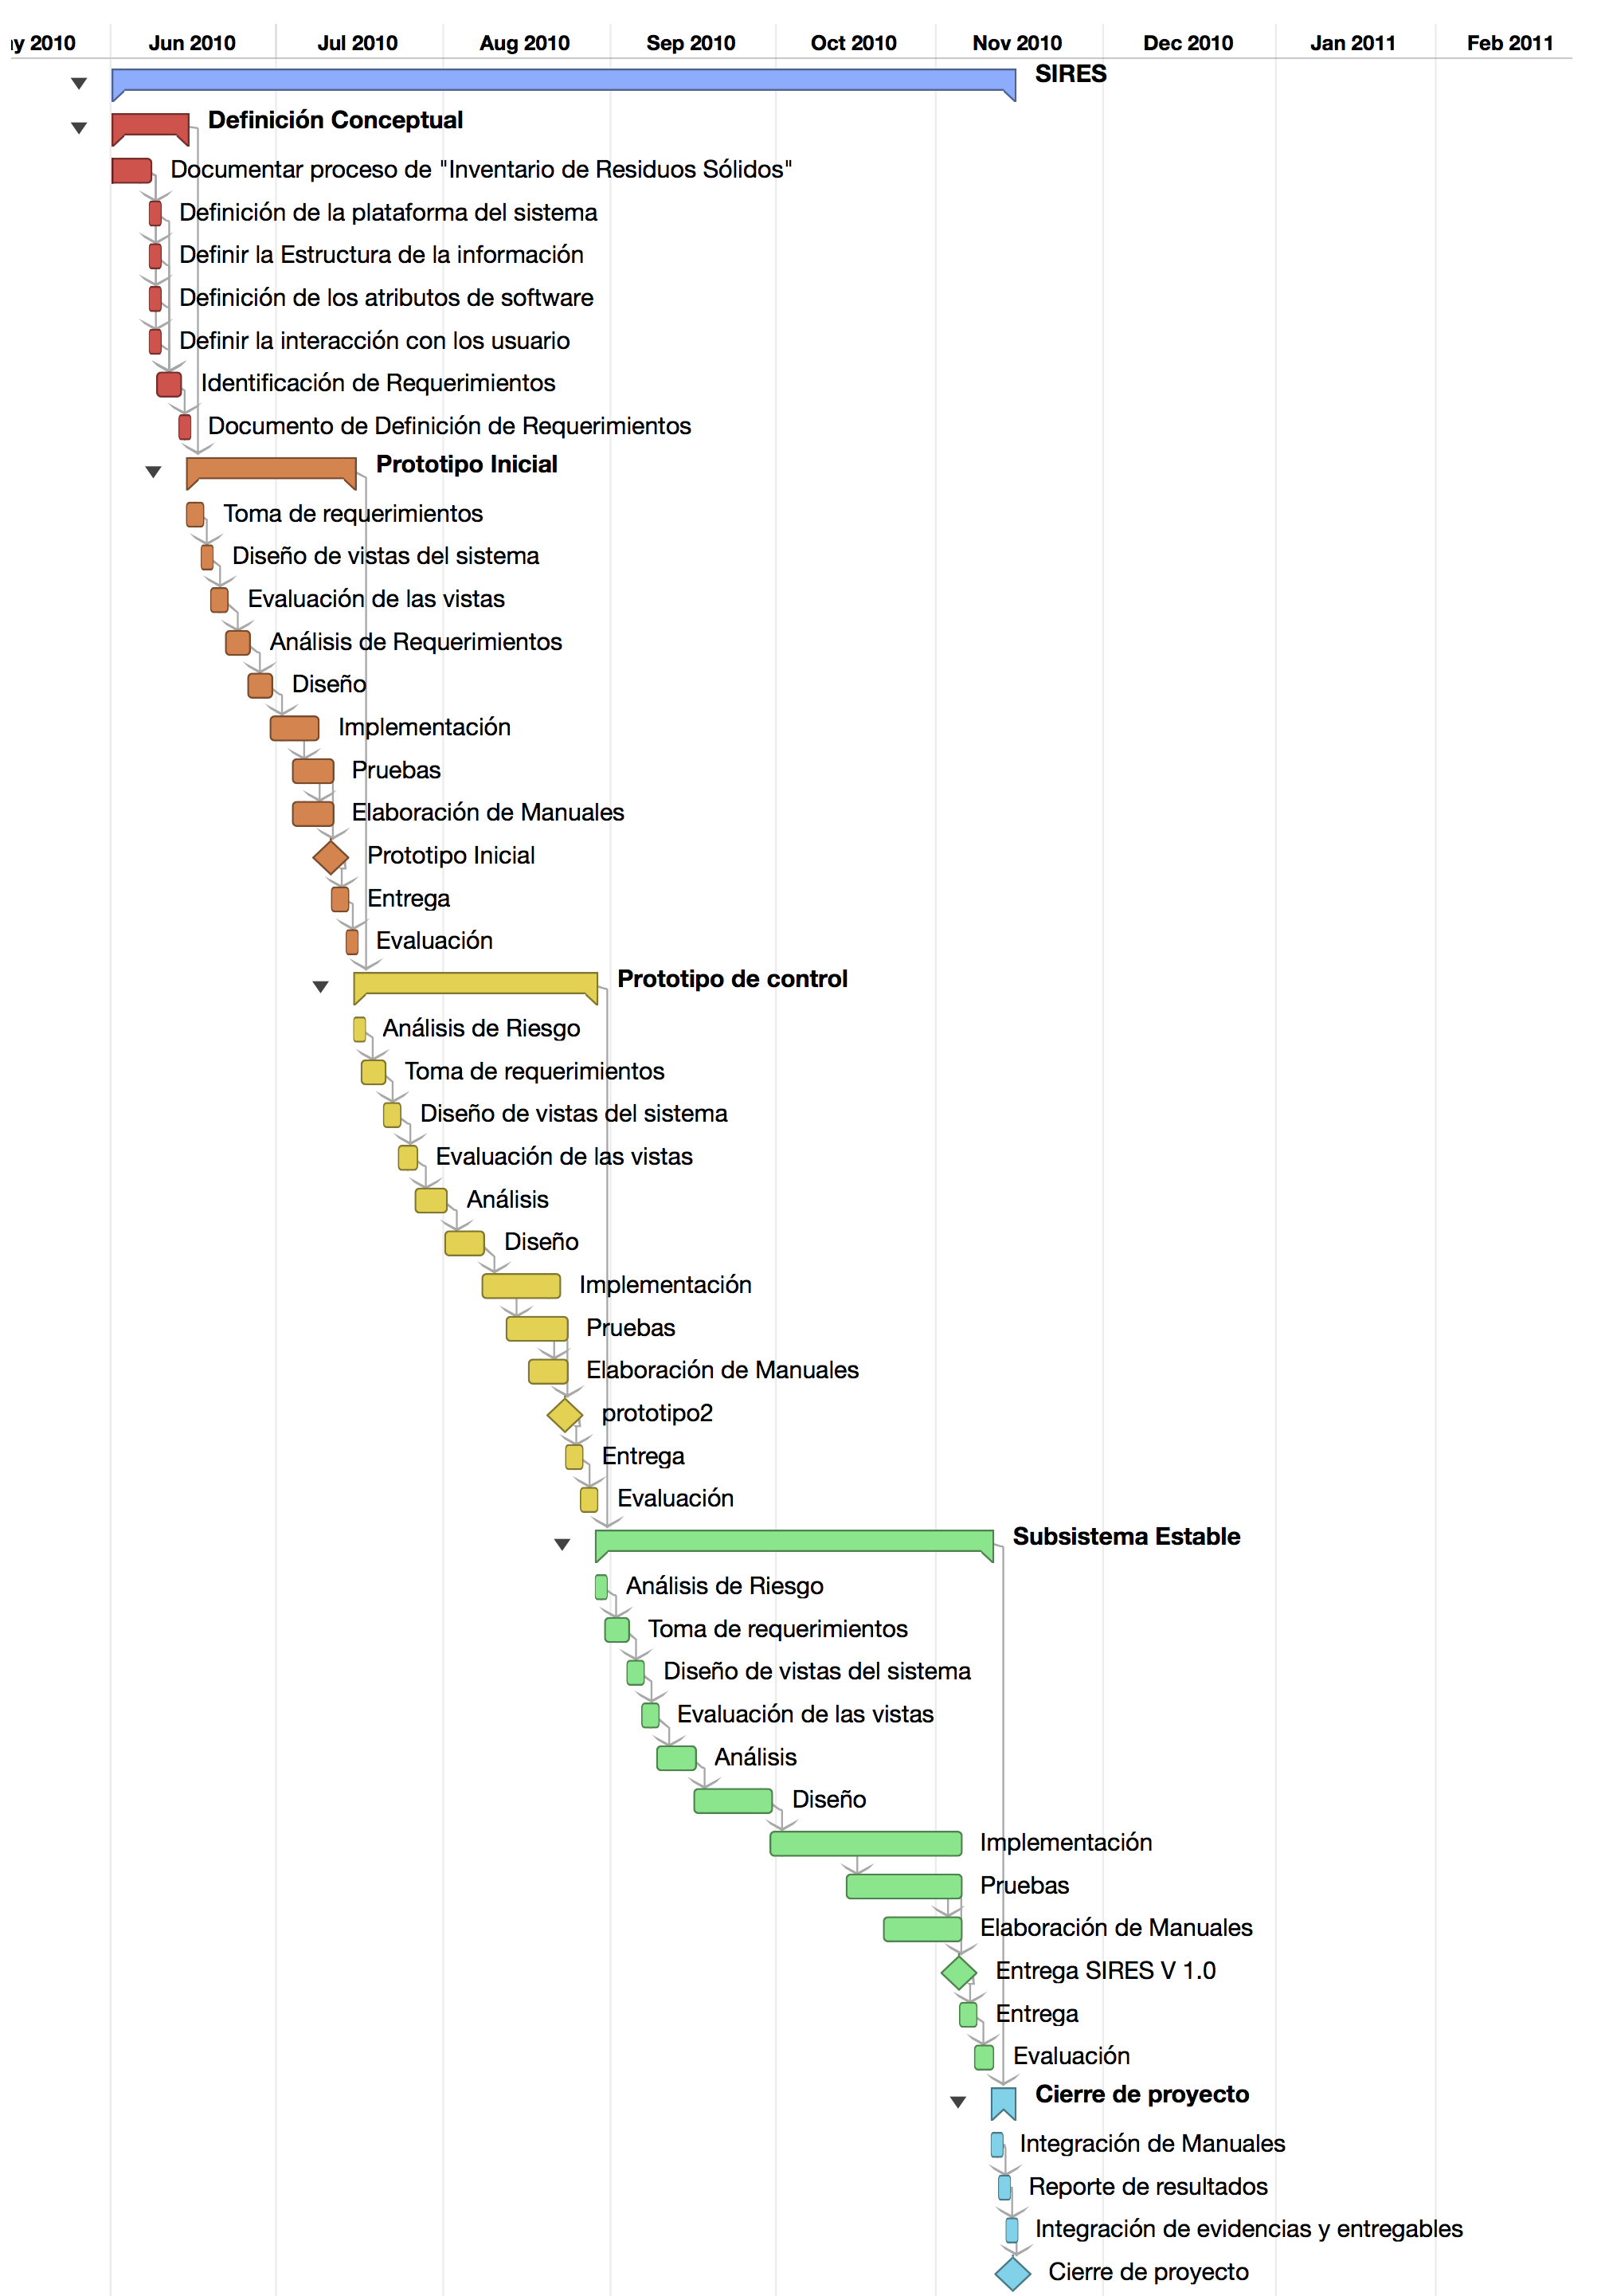
\includegraphics[width=.8\textwidth]{images/plan}}
		\caption{Plan de trabajo del proyecto}
		\label{fig:plan}
	\end{center}
\end{figure}

